\documentclass{report}

%%%%%%%%%%%%%%%%%%%%%%%%%%%%%%%%%
% PACKAGE IMPORTS
%%%%%%%%%%%%%%%%%%%%%%%%%%%%%%%%%

\usepackage[tmargin=2cm,rmargin=1in,lmargin=1in,margin=0.85in,bmargin=2cm,footskip=.2in]{geometry}
\usepackage{amsmath,amsfonts,amsthm,amssymb,mathtools}
\usepackage[varbb]{newpxmath}
\usepackage{xfrac}
\usepackage[makeroom]{cancel}
\usepackage{mathtools}
\usepackage{bookmark}
\usepackage{enumitem}
\usepackage{hyperref,theoremref}
\hypersetup{
	pdftitle={Assignment},
	colorlinks=true, linkcolor=doc!90,
	bookmarksnumbered=true,
	bookmarksopen=true
}
\usepackage[most,many,breakable]{tcolorbox}
\usepackage{xcolor}
\usepackage{varwidth}
\usepackage{varwidth}
\usepackage{etoolbox}
%\usepackage{authblk}
\usepackage{nameref}
\usepackage{multicol,array}
\usepackage{tikz-cd}
\usepackage[ruled,vlined,linesnumbered]{algorithm2e}
\usepackage{comment} % enables the use of multi-line comments (\ifx \fi) 
\usepackage{import}
\usepackage{xifthen}
\usepackage{pdfpages}
\usepackage{transparent}

\newcommand\mycommfont[1]{\footnotesize\ttfamily\textcolor{blue}{#1}}
\SetCommentSty{mycommfont}
\newcommand{\incfig}[1]{%
    \def\svgwidth{\columnwidth}
    \import{./figures/}{#1.pdf_tex}
}

\usepackage{tikzsymbols}
\renewcommand\qedsymbol{$\Laughey$}


%\usepackage{import}
%\usepackage{xifthen}
%\usepackage{pdfpages}
%\usepackage{transparent}


%%%%%%%%%%%%%%%%%%%%%%%%%%%%%%
% SELF MADE COLORS
%%%%%%%%%%%%%%%%%%%%%%%%%%%%%%



\definecolor{myg}{RGB}{56, 140, 70}
\definecolor{myb}{RGB}{45, 111, 177}
\definecolor{myr}{RGB}{199, 68, 64}
\definecolor{mytheorembg}{HTML}{F2F2F9}
\definecolor{mytheoremfr}{HTML}{00007B}
\definecolor{mylenmabg}{HTML}{FFFAF8}
\definecolor{mylenmafr}{HTML}{983b0f}
\definecolor{mypropbg}{HTML}{f2fbfc}
\definecolor{mypropfr}{HTML}{191971}
\definecolor{myexamplebg}{HTML}{F2FBF8}
\definecolor{myexamplefr}{HTML}{88D6D1}
\definecolor{myexampleti}{HTML}{2A7F7F}
\definecolor{mydefinitbg}{HTML}{E5E5FF}
\definecolor{mydefinitfr}{HTML}{3F3FA3}
\definecolor{notesgreen}{RGB}{0,162,0}
\definecolor{myp}{RGB}{197, 92, 212}
\definecolor{mygr}{HTML}{2C3338}
\definecolor{myred}{RGB}{127,0,0}
\definecolor{myyellow}{RGB}{169,121,69}
\definecolor{myexercisebg}{HTML}{F2FBF8}
\definecolor{myexercisefg}{HTML}{88D6D1}


%%%%%%%%%%%%%%%%%%%%%%%%%%%%
% TCOLORBOX SETUPS
%%%%%%%%%%%%%%%%%%%%%%%%%%%%

\setlength{\parindent}{1cm}
%================================
% THEOREM BOX
%================================

\tcbuselibrary{theorems,skins,hooks}
\newtcbtheorem[number within=section]{Theorem}{Theorem}
{%
	enhanced,
	breakable,
	colback = mytheorembg,
	frame hidden,
	boxrule = 0sp,
	borderline west = {2pt}{0pt}{mytheoremfr},
	sharp corners,
	detach title,
	before upper = \tcbtitle\par\smallskip,
	coltitle = mytheoremfr,
	fonttitle = \bfseries\sffamily,
	description font = \mdseries,
	separator sign none,
	segmentation style={solid, mytheoremfr},
}
{th}

\tcbuselibrary{theorems,skins,hooks}
\newtcbtheorem[number within=chapter]{theorem}{Theorem}
{%
	enhanced,
	breakable,
	colback = mytheorembg,
	frame hidden,
	boxrule = 0sp,
	borderline west = {2pt}{0pt}{mytheoremfr},
	sharp corners,
	detach title,
	before upper = \tcbtitle\par\smallskip,
	coltitle = mytheoremfr,
	fonttitle = \bfseries\sffamily,
	description font = \mdseries,
	separator sign none,
	segmentation style={solid, mytheoremfr},
}
{th}


\tcbuselibrary{theorems,skins,hooks}
\newtcolorbox{Theoremcon}
{%
	enhanced
	,breakable
	,colback = mytheorembg
	,frame hidden
	,boxrule = 0sp
	,borderline west = {2pt}{0pt}{mytheoremfr}
	,sharp corners
	,description font = \mdseries
	,separator sign none
}

%================================
% Corollery
%================================

\tcbuselibrary{theorems,skins,hooks}
\newtcbtheorem[number within=section]{Corollary}{}
{%
	enhanced
	,breakable
	,colback = myp!10
	,frame hidden
	,boxrule = 0sp
	,borderline west = {2pt}{0pt}{myp!85!black}
	,sharp corners
	,detach title
	,before upper = \tcbtitle\par\smallskip
	,coltitle = myp!85!black
	,fonttitle = \bfseries\sffamily
	,description font = \mdseries
	,separator sign none
	,segmentation style={solid, myp!85!black}
}
{th}
\tcbuselibrary{theorems,skins,hooks}
\newtcbtheorem[number within=chapter]{corollary}{Corollary}
{%
	enhanced
	,breakable
	,colback = myp!10
	,frame hidden
	,boxrule = 0sp
	,borderline west = {2pt}{0pt}{myp!85!black}
	,sharp corners
	,detach title
	,before upper = \tcbtitle\par\smallskip
	,coltitle = myp!85!black
	,fonttitle = \bfseries\sffamily
	,description font = \mdseries
	,separator sign none
	,segmentation style={solid, myp!85!black}
}
{th}


%================================
% LENMA
%================================

\tcbuselibrary{theorems,skins,hooks}
\newtcbtheorem[number within=section]{Lenma}{Lenma}
{%
	enhanced,
	breakable,
	colback = mylenmabg,
	frame hidden,
	boxrule = 0sp,
	borderline west = {2pt}{0pt}{mylenmafr},
	sharp corners,
	detach title,
	before upper = \tcbtitle\par\smallskip,
	coltitle = mylenmafr,
	fonttitle = \bfseries\sffamily,
	description font = \mdseries,
	separator sign none,
	segmentation style={solid, mylenmafr},
}
{th}

\tcbuselibrary{theorems,skins,hooks}
\newtcbtheorem[number within=chapter]{lenma}{Lenma}
{%
	enhanced,
	breakable,
	colback = mylenmabg,
	frame hidden,
	boxrule = 0sp,
	borderline west = {2pt}{0pt}{mylenmafr},
	sharp corners,
	detach title,
	before upper = \tcbtitle\par\smallskip,
	coltitle = mylenmafr,
	fonttitle = \bfseries\sffamily,
	description font = \mdseries,
	separator sign none,
	segmentation style={solid, mylenmafr},
}
{th}

%================================
% Formula 
%================================

\tcbuselibrary{theorems,skins,hooks}
\newtcbtheorem[no counter]{Frm}{}
{%
	enhanced,
	breakable,
	colback = mypropbg,
	frame hidden,
	boxrule = 0sp,
	borderline west = {2pt}{0pt}{mypropfr},
	sharp corners,
	detach title,
	before upper = \tcbtitle\par\smallskip,
	coltitle = mypropfr,
	fonttitle = \bfseries\sffamily,
	description font = \mdseries,
	separator sign none,
	segmentation style={solid, mypropfr},
}
{th}

%================================
% PROPOSITION
%================================

\tcbuselibrary{theorems,skins,hooks}
\newtcbtheorem[number within=section]{Prop}{Proposition}
{%
	enhanced,
	breakable,
	colback = mypropbg,
	frame hidden,
	boxrule = 0sp,
	borderline west = {2pt}{0pt}{mypropfr},
	sharp corners,
	detach title,
	before upper = \tcbtitle\par\smallskip,
	coltitle = mypropfr,
	fonttitle = \bfseries\sffamily,
	description font = \mdseries,
	separator sign none,
	segmentation style={solid, mypropfr},
}
{th}

\tcbuselibrary{theorems,skins,hooks}
\newtcbtheorem[number within=chapter]{prop}{Proposition}
{%
	enhanced,
	breakable,
	colback = mypropbg,
	frame hidden,
	boxrule = 0sp,
	borderline west = {2pt}{0pt}{mypropfr},
	sharp corners,
	detach title,
	before upper = \tcbtitle\par\smallskip,
	coltitle = mypropfr,
	fonttitle = \bfseries\sffamily,
	description font = \mdseries,
	separator sign none,
	segmentation style={solid, mypropfr},
}
{th}


%================================
% CLAIM
%================================

\tcbuselibrary{theorems,skins,hooks}
\newtcbtheorem[number within=section]{claim}{Claim}
{%
	enhanced
	,breakable
	,colback = myg!10
	,frame hidden
	,boxrule = 0sp
	,borderline west = {2pt}{0pt}{myg}
	,sharp corners
	,detach title
	,before upper = \tcbtitle\par\smallskip
	,coltitle = myg!85!black
	,fonttitle = \bfseries\sffamily
	,description font = \mdseries
	,separator sign none
	,segmentation style={solid, myg!85!black}
}
{th}



%================================
% Exercise
%================================

\tcbuselibrary{theorems,skins,hooks}
\newtcbtheorem[number within=section]{Exercise}{Exercise}
{%
	enhanced,
	breakable,
	colback = myexercisebg,
	frame hidden,
	boxrule = 0sp,
	borderline west = {2pt}{0pt}{myexercisefg},
	sharp corners,
	detach title,
	before upper = \tcbtitle\par\smallskip,
	coltitle = myexercisefg,
	fonttitle = \bfseries\sffamily,
	description font = \mdseries,
	separator sign none,
	segmentation style={solid, myexercisefg},
}
{th}

\tcbuselibrary{theorems,skins,hooks}
\newtcbtheorem[number within=chapter]{exercise}{Exercise}
{%
	enhanced,
	breakable,
	colback = myexercisebg,
	frame hidden,
	boxrule = 0sp,
	borderline west = {2pt}{0pt}{myexercisefg},
	sharp corners,
	detach title,
	before upper = \tcbtitle\par\smallskip,
	coltitle = myexercisefg,
	fonttitle = \bfseries\sffamily,
	description font = \mdseries,
	separator sign none,
	segmentation style={solid, myexercisefg},
}
{th}

%================================
% EXAMPLE BOX
%================================

\newtcbtheorem[number within=section]{Example}{Priklad}
{%
	colback = myexamplebg
	,breakable
	,colframe = myexamplefr
	,coltitle = myexampleti
	,boxrule = 1pt
	,sharp corners
	,detach title
	,before upper=\tcbtitle\par\smallskip
	,fonttitle = \bfseries
	,description font = \mdseries
	,separator sign none
	,description delimiters parenthesis
}
{ex}

\newtcbtheorem[number within=chapter]{example}{Example}
{%
	colback = myexamplebg
	,breakable
	,colframe = myexamplefr
	,coltitle = myexampleti
	,boxrule = 1pt
	,sharp corners
	,detach title
	,before upper=\tcbtitle\par\smallskip
	,fonttitle = \bfseries
	,description font = \mdseries
	,separator sign none
	,description delimiters parenthesis
}
{ex}

%================================
% DEFINITION BOX
%================================

\newtcbtheorem[number within=section]{Definition}{Definition}{enhanced,
	before skip=2mm,after skip=2mm, colback=red!5,colframe=red!80!black,boxrule=0.5mm,
	attach boxed title to top left={xshift=1cm,yshift*=1mm-\tcboxedtitleheight}, varwidth boxed title*=-3cm,
	boxed title style={frame code={
					\path[fill=tcbcolback]
					([yshift=-1mm,xshift=-1mm]frame.north west)
					arc[start angle=0,end angle=180,radius=1mm]
					([yshift=-1mm,xshift=1mm]frame.north east)
					arc[start angle=180,end angle=0,radius=1mm];
					\path[left color=tcbcolback!60!black,right color=tcbcolback!60!black,
						middle color=tcbcolback!80!black]
					([xshift=-2mm]frame.north west) -- ([xshift=2mm]frame.north east)
					[rounded corners=1mm]-- ([xshift=1mm,yshift=-1mm]frame.north east)
					-- (frame.south east) -- (frame.south west)
					-- ([xshift=-1mm,yshift=-1mm]frame.north west)
					[sharp corners]-- cycle;
				},interior engine=empty,
		},
	fonttitle=\bfseries,
	title={#2},#1}{def}
\newtcbtheorem[number within=chapter]{definition}{Definition}{enhanced,
	before skip=2mm,after skip=2mm, colback=red!5,colframe=red!80!black,boxrule=0.5mm,
	attach boxed title to top left={xshift=1cm,yshift*=1mm-\tcboxedtitleheight}, varwidth boxed title*=-3cm,
	boxed title style={frame code={
					\path[fill=tcbcolback]
					([yshift=-1mm,xshift=-1mm]frame.north west)
					arc[start angle=0,end angle=180,radius=1mm]
					([yshift=-1mm,xshift=1mm]frame.north east)
					arc[start angle=180,end angle=0,radius=1mm];
					\path[left color=tcbcolback!60!black,right color=tcbcolback!60!black,
						middle color=tcbcolback!80!black]
					([xshift=-2mm]frame.north west) -- ([xshift=2mm]frame.north east)
					[rounded corners=1mm]-- ([xshift=1mm,yshift=-1mm]frame.north east)
					-- (frame.south east) -- (frame.south west)
					-- ([xshift=-1mm,yshift=-1mm]frame.north west)
					[sharp corners]-- cycle;
				},interior engine=empty,
		},
	fonttitle=\bfseries,
	title={#2},#1}{def}



%================================
% Solution BOX
%================================

\makeatletter
\newtcbtheorem{question}{Question}{enhanced,
	breakable,
	colback=white,
	colframe=myb!80!black,
	attach boxed title to top left={yshift*=-\tcboxedtitleheight},
	fonttitle=\bfseries,
	title={#2},
	boxed title size=title,
	boxed title style={%
			sharp corners,
			rounded corners=northwest,
			colback=tcbcolframe,
			boxrule=0pt,
		},
	underlay boxed title={%
			\path[fill=tcbcolframe] (title.south west)--(title.south east)
			to[out=0, in=180] ([xshift=5mm]title.east)--
			(title.center-|frame.east)
			[rounded corners=\kvtcb@arc] |-
			(frame.north) -| cycle;
		},
	#1
}{def}
\makeatother

%================================
% SOLUTION BOX
%================================

\makeatletter
\newtcolorbox{solution}{enhanced,
	breakable,
	colback=white,
	colframe=myg!80!black,
	attach boxed title to top left={yshift*=-\tcboxedtitleheight},
	title=Solution,
	boxed title size=title,
	boxed title style={%
			sharp corners,
			rounded corners=northwest,
			colback=tcbcolframe,
			boxrule=0pt,
		},
	underlay boxed title={%
			\path[fill=tcbcolframe] (title.south west)--(title.south east)
			to[out=0, in=180] ([xshift=5mm]title.east)--
			(title.center-|frame.east)
			[rounded corners=\kvtcb@arc] |-
			(frame.north) -| cycle;
		},
}
\makeatother

%================================
% Question BOX
%================================

\makeatletter
\newtcbtheorem{qstion}{Question}{enhanced,
	breakable,
	colback=white,
	colframe=mygr,
	attach boxed title to top left={yshift*=-\tcboxedtitleheight},
	fonttitle=\bfseries,
	title={#2},
	boxed title size=title,
	boxed title style={%
			sharp corners,
			rounded corners=northwest,
			colback=tcbcolframe,
			boxrule=0pt,
		},
	underlay boxed title={%
			\path[fill=tcbcolframe] (title.south west)--(title.south east)
			to[out=0, in=180] ([xshift=5mm]title.east)--
			(title.center-|frame.east)
			[rounded corners=\kvtcb@arc] |-
			(frame.north) -| cycle;
		},
	#1
}{def}
\makeatother

\newtcbtheorem[number within=chapter]{wconc}{Wrong Concept}{
	breakable,
	enhanced,
	colback=white,
	colframe=myr,
	arc=0pt,
	outer arc=0pt,
	fonttitle=\bfseries\sffamily\large,
	colbacktitle=myr,
	attach boxed title to top left={},
	boxed title style={
			enhanced,
			skin=enhancedfirst jigsaw,
			arc=3pt,
			bottom=0pt,
			interior style={fill=myr}
		},
	#1
}{def}



%================================
% NOTE BOX
%================================

\usetikzlibrary{arrows,calc,shadows.blur}
\tcbuselibrary{skins}
\newtcolorbox{note}[1][]{%
	enhanced jigsaw,
	colback=gray!20!white,%
	colframe=gray!80!black,
	size=small,
	boxrule=1pt,
	title=\textbf{Note:-},
	halign title=flush center,
	coltitle=black,
	breakable,
	drop shadow=black!50!white,
	attach boxed title to top left={xshift=1cm,yshift=-\tcboxedtitleheight/2,yshifttext=-\tcboxedtitleheight/2},
	minipage boxed title=1.5cm,
	boxed title style={%
			colback=white,
			size=fbox,
			boxrule=1pt,
			boxsep=2pt,
			underlay={%
					\coordinate (dotA) at ($(interior.west) + (-0.5pt,0)$);
					\coordinate (dotB) at ($(interior.east) + (0.5pt,0)$);
					\begin{scope}
						\clip (interior.north west) rectangle ([xshift=3ex]interior.east);
						\filldraw [white, blur shadow={shadow opacity=60, shadow yshift=-.75ex}, rounded corners=2pt] (interior.north west) rectangle (interior.south east);
					\end{scope}
					\begin{scope}[gray!80!black]
						\fill (dotA) circle (2pt);
						\fill (dotB) circle (2pt);
					\end{scope}
				},
		},
	#1,
}

%%%%%%%%%%%%%%%%%%%%%%%%%%%%%%
% SELF MADE COMMANDS
%%%%%%%%%%%%%%%%%%%%%%%%%%%%%%


\newcommand{\thm}[2]{\begin{Theorem}{#1}{}#2\end{Theorem}}
\newcommand{\cor}[2]{\begin{Corollary}{#1}{}#2\end{Corollary}}
\newcommand{\mlenma}[2]{\begin{Lenma}{#1}{}#2\end{Lenma}}
\newcommand{\mprop}[2]{\begin{Prop}{#1}{}#2\end{Prop}}
\newcommand{\clm}[3]{\begin{claim}{#1}{#2}#3\end{claim}}
\newcommand{\wc}[2]{\begin{wconc}{#1}{}\setlength{\parindent}{1cm}#2\end{wconc}}
\newcommand{\thmcon}[1]{\begin{Theoremcon}{#1}\end{Theoremcon}}
\newcommand{\ex}[2]{\begin{Example}{#1}{}#2\end{Example}}
\newcommand{\dfn}[2]{\begin{Definition}[colbacktitle=red!75!black]{#1}{}#2\end{Definition}}
\newcommand{\dfnc}[2]{\begin{definition}[colbacktitle=red!75!black]{#1}{}#2\end{definition}}
\newcommand{\qs}[2]{\begin{question}{#1}{}#2\end{question}}
\newcommand{\pf}[2]{\begin{myproof}[#1]#2\end{myproof}}
\newcommand{\nt}[1]{\begin{note}#1\end{note}}

\newcommand{\frm}[1]{\begin{tcolorbox}[
	enhanced,
	breakable,
	colback = mypropbg,
	frame hidden,
	boxrule = 0sp,
	borderline west = {2pt}{0pt}{mypropfr},
	sharp corners,
]#1\end{tcolorbox}}

\newcommand{\law}[1]{\begin{tcolorbox}[
	enhanced,
	breakable,
	colback = myp!10,
	frame hidden,
	boxrule = 0sp,
	borderline west = {2pt}{0pt}{myp!85!black},
	sharp corners,
]#1\end{tcolorbox}}

\newcommand*\circled[1]{\tikz[baseline=(char.base)]{
		\node[shape=circle,draw,inner sep=1pt] (char) {#1};}}
\newcommand\getcurrentref[1]{%
	\ifnumequal{\value{#1}}{0}
	{??}
	{\the\value{#1}}%
}
\newcommand{\getCurrentSectionNumber}{\getcurrentref{section}}
\newenvironment{myproof}[1][\proofname]{%
	\proof[\bfseries #1: ]%
}{\endproof}

\newcommand{\mclm}[2]{\begin{myclaim}[#1]#2\end{myclaim}}
\newenvironment{myclaim}[1][\claimname]{\proof[\bfseries #1: ]}{}

\newcounter{mylabelcounter}

\makeatletter
\newcommand{\setword}[2]{%
	\phantomsection
	#1\def\@currentlabel{\unexpanded{#1}}\label{#2}%
}
\makeatother




\tikzset{
	symbol/.style={
			draw=none,
			every to/.append style={
					edge node={node [sloped, allow upside down, auto=false]{$#1$}}}
		}
}


% deliminators
\DeclarePairedDelimiter{\abs}{\lvert}{\rvert}
\DeclarePairedDelimiter{\norm}{\lVert}{\rVert}

\DeclarePairedDelimiter{\ceil}{\lceil}{\rceil}
\DeclarePairedDelimiter{\floor}{\lfloor}{\rfloor}
\DeclarePairedDelimiter{\round}{\lfloor}{\rceil}

\newsavebox\diffdbox
\newcommand{\slantedromand}{{\mathpalette\makesl{d}}}
\newcommand{\makesl}[2]{%
\begingroup
\sbox{\diffdbox}{$\mathsurround=0pt#1\mathrm{#2}$}%
\pdfsave
\pdfsetmatrix{1 0 0.2 1}%
\rlap{\usebox{\diffdbox}}%
\pdfrestore
\hskip\wd\diffdbox
\endgroup
}
\newcommand{\dd}[1][]{\ensuremath{\mathop{}\!\ifstrempty{#1}{%
\slantedromand\@ifnextchar^{\hspace{0.2ex}}{\hspace{0.1ex}}}%
{\slantedromand\hspace{0.2ex}^{#1}}}}
\ProvideDocumentCommand\dv{o m g}{%
  \ensuremath{%
    \IfValueTF{#3}{%
      \IfNoValueTF{#1}{%
        \frac{\dd #2}{\dd #3}%
      }{%
        \frac{\dd^{#1} #2}{\dd #3^{#1}}%
      }%
    }{%
      \IfNoValueTF{#1}{%
        \frac{\dd}{\dd #2}%
      }{%
        \frac{\dd^{#1}}{\dd #2^{#1}}%
      }%
    }%
  }%
}
\providecommand*{\pdv}[3][]{\frac{\partial^{#1}#2}{\partial#3^{#1}}}
%  - others
\DeclareMathOperator{\Lap}{\mathcal{L}}
\DeclareMathOperator{\Var}{Var} % varience
\DeclareMathOperator{\Cov}{Cov} % covarience
\DeclareMathOperator{\E}{E} % expected

% Since the amsthm package isn't loaded

% I prefer the slanted \leq
\let\oldleq\leq % save them in case they're every wanted
\let\oldgeq\geq
\renewcommand{\leq}{\leqslant}
\renewcommand{\geq}{\geqslant}

% % redefine matrix env to allow for alignment, use r as default
% \renewcommand*\env@matrix[1][r]{\hskip -\arraycolsep
%     \let\@ifnextchar\new@ifnextchar
%     \array{*\c@MaxMatrixCols #1}}


%\usepackage{framed}
%\usepackage{titletoc}
%\usepackage{etoolbox}
%\usepackage{lmodern}


%\patchcmd{\tableofcontents}{\contentsname}{\sffamily\contentsname}{}{}

%\renewenvironment{leftbar}
%{\def\FrameCommand{\hspace{6em}%
%		{\color{myyellow}\vrule width 2pt depth 6pt}\hspace{1em}}%
%	\MakeFramed{\parshape 1 0cm \dimexpr\textwidth-6em\relax\FrameRestore}\vskip2pt%
%}
%{\endMakeFramed}

%\titlecontents{chapter}
%[0em]{\vspace*{2\baselineskip}}
%{\parbox{4.5em}{%
%		\hfill\Huge\sffamily\bfseries\color{myred}\thecontentspage}%
%	\vspace*{-2.3\baselineskip}\leftbar\textsc{\small\chaptername~\thecontentslabel}\\\sffamily}
%{}{\endleftbar}
%\titlecontents{section}
%[8.4em]
%{\sffamily\contentslabel{3em}}{}{}
%{\hspace{0.5em}\nobreak\itshape\color{myred}\contentspage}
%\titlecontents{subsection}
%[8.4em]
%{\sffamily\contentslabel{3em}}{}{}  
%{\hspace{0.5em}\nobreak\itshape\color{myred}\contentspage}



%%%%%%%%%%%%%%%%%%%%%%%%%%%%%%%%%%%%%%%%%%%
% TABLE OF CONTENTS
%%%%%%%%%%%%%%%%%%%%%%%%%%%%%%%%%%%%%%%%%%%

\usepackage{tikz}
\definecolor{doc}{RGB}{0,60,110}
\usepackage{titletoc}
\contentsmargin{0cm}
\titlecontents{chapter}[3.7pc]
{\addvspace{30pt}%
	\begin{tikzpicture}[remember picture, overlay]%
		\draw[fill=doc!60,draw=doc!60] (-7,-.1) rectangle (-0.9,.5);%
		\pgftext[left,x=-3.5cm,y=0.2cm]{\color{white}\Large\sc\bfseries Chapter\ \thecontentslabel};%
	\end{tikzpicture}\color{doc!60}\large\sc\bfseries}%
{}
{}
{\;\titlerule\;\large\sc\bfseries Page \thecontentspage
	\begin{tikzpicture}[remember picture, overlay]
		\draw[fill=doc!60,draw=doc!60] (2pt,0) rectangle (4,0.1pt);
	\end{tikzpicture}}%
\titlecontents{section}[3.7pc]
{\addvspace{2pt}}
{\contentslabel[\thecontentslabel]{2pc}}
{}
{\hfill\small \thecontentspage}
[]
\titlecontents*{subsection}[3.7pc]
{\addvspace{-1pt}\small}
{}
{}
{\ --- \small\thecontentspage}
[ \textbullet\ ][]

\makeatletter
\renewcommand{\tableofcontents}{%
	\chapter*{%
	  \vspace*{-20\p@}%
	  \begin{tikzpicture}[remember picture, overlay]%
		  \pgftext[right,x=15cm,y=0.2cm]{\color{doc!60}\Huge\sc\bfseries \contentsname};%
		  \draw[fill=doc!60,draw=doc!60] (13,-.75) rectangle (20,1);%
		  \clip (13,-.75) rectangle (20,1);
		  \pgftext[right,x=15cm,y=0.2cm]{\color{white}\Huge\sc\bfseries \contentsname};%
	  \end{tikzpicture}}%
	\@starttoc{toc}}
\makeatother


%From M275 "Topology" at SJSU
\newcommand{\id}{\mathrm{id}}
\newcommand{\taking}[1]{\xrightarrow{#1}}
\newcommand{\inv}{^{-1}}

%From M170 "Introduction to Graph Theory" at SJSU
\DeclareMathOperator{\diam}{diam}
\DeclareMathOperator{\ord}{ord}
\newcommand{\defeq}{\overset{\mathrm{def}}{=}}

%From the USAMO .tex files
\newcommand{\ts}{\textsuperscript}
\newcommand{\dg}{^\circ}
\newcommand{\ii}{\item}

% % From Math 55 and Math 145 at Harvard
% \newenvironment{subproof}[1][Proof]{%
% \begin{proof}[#1] \renewcommand{\qedsymbol}{$\blacksquare$}}%
% {\end{proof}}

\newcommand{\liff}{\leftrightarrow}
\newcommand{\lthen}{\rightarrow}
\newcommand{\opname}{\operatorname}
\newcommand{\surjto}{\twoheadrightarrow}
\newcommand{\injto}{\hookrightarrow}
\newcommand{\On}{\mathrm{On}} % ordinals
\DeclareMathOperator{\img}{im} % Image
\DeclareMathOperator{\Img}{Im} % Image
\DeclareMathOperator{\coker}{coker} % Cokernel
\DeclareMathOperator{\Coker}{Coker} % Cokernel
\DeclareMathOperator{\Ker}{Ker} % Kernel
\DeclareMathOperator{\rank}{rank}
\DeclareMathOperator{\Spec}{Spec} % spectrum
\DeclareMathOperator{\Tr}{Tr} % trace
\DeclareMathOperator{\pr}{pr} % projection
\DeclareMathOperator{\ext}{ext} % extension
\DeclareMathOperator{\pred}{pred} % predecessor
\DeclareMathOperator{\dom}{dom} % domain
\DeclareMathOperator{\ran}{ran} % range
\DeclareMathOperator{\Hom}{Hom} % homomorphism
\DeclareMathOperator{\Mor}{Mor} % morphisms
\DeclareMathOperator{\End}{End} % endomorphism

\newcommand{\eps}{\epsilon}
\newcommand{\veps}{\varepsilon}
\newcommand{\ol}{\overline}
\newcommand{\ul}{\underline}
\newcommand{\wt}{\widetilde}
\newcommand{\wh}{\widehat}
\newcommand{\vocab}[1]{\textbf{\color{blue} #1}}
\providecommand{\half}{\frac{1}{2}}
\newcommand{\dang}{\measuredangle} %% Directed angle
\newcommand{\ray}[1]{\overrightarrow{#1}}
\newcommand{\seg}[1]{\overline{#1}}
\newcommand{\arc}[1]{\wideparen{#1}}
\DeclareMathOperator{\cis}{cis}
\DeclareMathOperator*{\lcm}{lcm}
\DeclareMathOperator*{\argmin}{arg min}
\DeclareMathOperator*{\argmax}{arg max}
\newcommand{\cycsum}{\sum_{\mathrm{cyc}}}
\newcommand{\symsum}{\sum_{\mathrm{sym}}}
\newcommand{\cycprod}{\prod_{\mathrm{cyc}}}
\newcommand{\symprod}{\prod_{\mathrm{sym}}}
\newcommand{\Qed}{\begin{flushright}\qed\end{flushright}}
\newcommand{\parinn}{\setlength{\parindent}{1cm}}
\newcommand{\parinf}{\setlength{\parindent}{0cm}}
% \newcommand{\norm}{\|\cdot\|}
\newcommand{\inorm}{\norm_{\infty}}
\newcommand{\opensets}{\{V_{\alpha}\}_{\alpha\in I}}
\newcommand{\oset}{V_{\alpha}}
\newcommand{\opset}[1]{V_{\alpha_{#1}}}
\newcommand{\lub}{\text{lub}}
\newcommand{\del}[2]{\frac{\partial #1}{\partial #2}}
\newcommand{\Del}[3]{\frac{\partial^{#1} #2}{\partial^{#1} #3}}
\newcommand{\deld}[2]{\dfrac{\partial #1}{\partial #2}}
\newcommand{\Deld}[3]{\dfrac{\partial^{#1} #2}{\partial^{#1} #3}}
\newcommand{\lm}{\lambda}
\newcommand{\uin}{\mathbin{\rotatebox[origin=c]{90}{$\in$}}}
\newcommand{\usubset}{\mathbin{\rotatebox[origin=c]{90}{$\subset$}}}
\newcommand{\lt}{\left}
\newcommand{\rt}{\right}
\newcommand{\bs}[1]{\boldsymbol{#1}}
\newcommand{\exs}{\exists}
\newcommand{\st}{\strut}
\newcommand{\dps}[1]{\displaystyle{#1}}

\newcommand{\sol}{\setlength{\parindent}{0cm}\textbf{\textit{Solution:}}\setlength{\parindent}{1cm} }
\newcommand{\solve}[1]{\setlength{\parindent}{0cm}\textbf{\textit{Solution: }}\setlength{\parindent}{1cm}#1 \Qed}

% Things Lie
\newcommand{\kb}{\mathfrak b}
\newcommand{\kg}{\mathfrak g}
\newcommand{\kh}{\mathfrak h}
\newcommand{\kn}{\mathfrak n}
\newcommand{\ku}{\mathfrak u}
\newcommand{\kz}{\mathfrak z}
\DeclareMathOperator{\Ext}{Ext} % Ext functor
\DeclareMathOperator{\Tor}{Tor} % Tor functor
\newcommand{\gl}{\opname{\mathfrak{gl}}} % frak gl group
\renewcommand{\sl}{\opname{\mathfrak{sl}}} % frak sl group chktex 6

% More script letters etc.
\newcommand{\SA}{\mathcal A}
\newcommand{\SB}{\mathcal B}
\newcommand{\SC}{\mathcal C}
\newcommand{\SF}{\mathcal F}
\newcommand{\SG}{\mathcal G}
\newcommand{\SH}{\mathcal H}
\newcommand{\OO}{\mathcal O}

\newcommand{\SCA}{\mathscr A}
\newcommand{\SCB}{\mathscr B}
\newcommand{\SCC}{\mathscr C}
\newcommand{\SCD}{\mathscr D}
\newcommand{\SCE}{\mathscr E}
\newcommand{\SCF}{\mathscr F}
\newcommand{\SCG}{\mathscr G}
\newcommand{\SCH}{\mathscr H}

% Mathfrak primes
\newcommand{\km}{\mathfrak m}
\newcommand{\kp}{\mathfrak p}
\newcommand{\kq}{\mathfrak q}

% number sets
\newcommand{\RR}[1][]{\ensuremath{\ifstrempty{#1}{\mathbb{R}}{\mathbb{R}^{#1}}}}
\newcommand{\NN}[1][]{\ensuremath{\ifstrempty{#1}{\mathbb{N}}{\mathbb{N}^{#1}}}}
\newcommand{\ZZ}[1][]{\ensuremath{\ifstrempty{#1}{\mathbb{Z}}{\mathbb{Z}^{#1}}}}
\newcommand{\QQ}[1][]{\ensuremath{\ifstrempty{#1}{\mathbb{Q}}{\mathbb{Q}^{#1}}}}
\newcommand{\CC}[1][]{\ensuremath{\ifstrempty{#1}{\mathbb{C}}{\mathbb{C}^{#1}}}}
\newcommand{\PP}[1][]{\ensuremath{\ifstrempty{#1}{\mathbb{P}}{\mathbb{P}^{#1}}}}
\newcommand{\HH}[1][]{\ensuremath{\ifstrempty{#1}{\mathbb{H}}{\mathbb{H}^{#1}}}}
\newcommand{\FF}[1][]{\ensuremath{\ifstrempty{#1}{\mathbb{F}}{\mathbb{F}^{#1}}}}
% expected value
\newcommand{\EE}{\ensuremath{\mathbb{E}}}
\newcommand{\charin}{\text{ char }}
\DeclareMathOperator{\sign}{sign}
\DeclareMathOperator{\Aut}{Aut}
\DeclareMathOperator{\Inn}{Inn}
\DeclareMathOperator{\Syl}{Syl}
\DeclareMathOperator{\Gal}{Gal}
\DeclareMathOperator{\GL}{GL} % General linear group
\DeclareMathOperator{\SL}{SL} % Special linear group

%---------------------------------------
% BlackBoard Math Fonts :-
%---------------------------------------

%Captital Letters
\newcommand{\bbA}{\mathbb{A}}	\newcommand{\bbB}{\mathbb{B}}
\newcommand{\bbC}{\mathbb{C}}	\newcommand{\bbD}{\mathbb{D}}
\newcommand{\bbE}{\mathbb{E}}	\newcommand{\bbF}{\mathbb{F}}
\newcommand{\bbG}{\mathbb{G}}	\newcommand{\bbH}{\mathbb{H}}
\newcommand{\bbI}{\mathbb{I}}	\newcommand{\bbJ}{\mathbb{J}}
\newcommand{\bbK}{\mathbb{K}}	\newcommand{\bbL}{\mathbb{L}}
\newcommand{\bbM}{\mathbb{M}}	\newcommand{\bbN}{\mathbb{N}}
\newcommand{\bbO}{\mathbb{O}}	\newcommand{\bbP}{\mathbb{P}}
\newcommand{\bbQ}{\mathbb{Q}}	\newcommand{\bbR}{\mathbb{R}}
\newcommand{\bbS}{\mathbb{S}}	\newcommand{\bbT}{\mathbb{T}}
\newcommand{\bbU}{\mathbb{U}}	\newcommand{\bbV}{\mathbb{V}}
\newcommand{\bbW}{\mathbb{W}}	\newcommand{\bbX}{\mathbb{X}}
\newcommand{\bbY}{\mathbb{Y}}	\newcommand{\bbZ}{\mathbb{Z}}

%---------------------------------------
% MathCal Fonts :-
%---------------------------------------

%Captital Letters
\newcommand{\mcA}{\mathcal{A}}	\newcommand{\mcB}{\mathcal{B}}
\newcommand{\mcC}{\mathcal{C}}	\newcommand{\mcD}{\mathcal{D}}
\newcommand{\mcE}{\mathcal{E}}	\newcommand{\mcF}{\mathcal{F}}
\newcommand{\mcG}{\mathcal{G}}	\newcommand{\mcH}{\mathcal{H}}
\newcommand{\mcI}{\mathcal{I}}	\newcommand{\mcJ}{\mathcal{J}}
\newcommand{\mcK}{\mathcal{K}}	\newcommand{\mcL}{\mathcal{L}}
\newcommand{\mcM}{\mathcal{M}}	\newcommand{\mcN}{\mathcal{N}}
\newcommand{\mcO}{\mathcal{O}}	\newcommand{\mcP}{\mathcal{P}}
\newcommand{\mcQ}{\mathcal{Q}}	\newcommand{\mcR}{\mathcal{R}}
\newcommand{\mcS}{\mathcal{S}}	\newcommand{\mcT}{\mathcal{T}}
\newcommand{\mcU}{\mathcal{U}}	\newcommand{\mcV}{\mathcal{V}}
\newcommand{\mcW}{\mathcal{W}}	\newcommand{\mcX}{\mathcal{X}}
\newcommand{\mcY}{\mathcal{Y}}	\newcommand{\mcZ}{\mathcal{Z}}


%---------------------------------------
% Bold Math Fonts :-
%---------------------------------------

%Captital Letters
\newcommand{\bmA}{\boldsymbol{A}}	\newcommand{\bmB}{\boldsymbol{B}}
\newcommand{\bmC}{\boldsymbol{C}}	\newcommand{\bmD}{\boldsymbol{D}}
\newcommand{\bmE}{\boldsymbol{E}}	\newcommand{\bmF}{\boldsymbol{F}}
\newcommand{\bmG}{\boldsymbol{G}}	\newcommand{\bmH}{\boldsymbol{H}}
\newcommand{\bmI}{\boldsymbol{I}}	\newcommand{\bmJ}{\boldsymbol{J}}
\newcommand{\bmK}{\boldsymbol{K}}	\newcommand{\bmL}{\boldsymbol{L}}
\newcommand{\bmM}{\boldsymbol{M}}	\newcommand{\bmN}{\boldsymbol{N}}
\newcommand{\bmO}{\boldsymbol{O}}	\newcommand{\bmP}{\boldsymbol{P}}
\newcommand{\bmQ}{\boldsymbol{Q}}	\newcommand{\bmR}{\boldsymbol{R}}
\newcommand{\bmS}{\boldsymbol{S}}	\newcommand{\bmT}{\boldsymbol{T}}
\newcommand{\bmU}{\boldsymbol{U}}	\newcommand{\bmV}{\boldsymbol{V}}
\newcommand{\bmW}{\boldsymbol{W}}	\newcommand{\bmX}{\boldsymbol{X}}
\newcommand{\bmY}{\boldsymbol{Y}}	\newcommand{\bmZ}{\boldsymbol{Z}}
%Small Letters
\newcommand{\bma}{\boldsymbol{a}}	\newcommand{\bmb}{\boldsymbol{b}}
\newcommand{\bmc}{\boldsymbol{c}}	\newcommand{\bmd}{\boldsymbol{d}}
\newcommand{\bme}{\boldsymbol{e}}	\newcommand{\bmf}{\boldsymbol{f}}
\newcommand{\bmg}{\boldsymbol{g}}	\newcommand{\bmh}{\boldsymbol{h}}
\newcommand{\bmi}{\boldsymbol{i}}	\newcommand{\bmj}{\boldsymbol{j}}
\newcommand{\bmk}{\boldsymbol{k}}	\newcommand{\bml}{\boldsymbol{l}}
\newcommand{\bmm}{\boldsymbol{m}}	\newcommand{\bmn}{\boldsymbol{n}}
\newcommand{\bmo}{\boldsymbol{o}}	\newcommand{\bmp}{\boldsymbol{p}}
\newcommand{\bmq}{\boldsymbol{q}}	\newcommand{\bmr}{\boldsymbol{r}}
\newcommand{\bms}{\boldsymbol{s}}	\newcommand{\bmt}{\boldsymbol{t}}
\newcommand{\bmu}{\boldsymbol{u}}	\newcommand{\bmv}{\boldsymbol{v}}
\newcommand{\bmw}{\boldsymbol{w}}	\newcommand{\bmx}{\boldsymbol{x}}
\newcommand{\bmy}{\boldsymbol{y}}	\newcommand{\bmz}{\boldsymbol{z}}

%---------------------------------------
% Scr Math Fonts :-
%---------------------------------------

\newcommand{\sA}{{\mathscr{A}}}   \newcommand{\sB}{{\mathscr{B}}}
\newcommand{\sC}{{\mathscr{C}}}   \newcommand{\sD}{{\mathscr{D}}}
\newcommand{\sE}{{\mathscr{E}}}   \newcommand{\sF}{{\mathscr{F}}}
\newcommand{\sG}{{\mathscr{G}}}   \newcommand{\sH}{{\mathscr{H}}}
\newcommand{\sI}{{\mathscr{I}}}   \newcommand{\sJ}{{\mathscr{J}}}
\newcommand{\sK}{{\mathscr{K}}}   \newcommand{\sL}{{\mathscr{L}}}
\newcommand{\sM}{{\mathscr{M}}}   \newcommand{\sN}{{\mathscr{N}}}
\newcommand{\sO}{{\mathscr{O}}}   \newcommand{\sP}{{\mathscr{P}}}
\newcommand{\sQ}{{\mathscr{Q}}}   \newcommand{\sR}{{\mathscr{R}}}
\newcommand{\sS}{{\mathscr{S}}}   \newcommand{\sT}{{\mathscr{T}}}
\newcommand{\sU}{{\mathscr{U}}}   \newcommand{\sV}{{\mathscr{V}}}
\newcommand{\sW}{{\mathscr{W}}}   \newcommand{\sX}{{\mathscr{X}}}
\newcommand{\sY}{{\mathscr{Y}}}   \newcommand{\sZ}{{\mathscr{Z}}}


%---------------------------------------
% Math Fraktur Font
%---------------------------------------

%Captital Letters
\newcommand{\mfA}{\mathfrak{A}}	\newcommand{\mfB}{\mathfrak{B}}
\newcommand{\mfC}{\mathfrak{C}}	\newcommand{\mfD}{\mathfrak{D}}
\newcommand{\mfE}{\mathfrak{E}}	\newcommand{\mfF}{\mathfrak{F}}
\newcommand{\mfG}{\mathfrak{G}}	\newcommand{\mfH}{\mathfrak{H}}
\newcommand{\mfI}{\mathfrak{I}}	\newcommand{\mfJ}{\mathfrak{J}}
\newcommand{\mfK}{\mathfrak{K}}	\newcommand{\mfL}{\mathfrak{L}}
\newcommand{\mfM}{\mathfrak{M}}	\newcommand{\mfN}{\mathfrak{N}}
\newcommand{\mfO}{\mathfrak{O}}	\newcommand{\mfP}{\mathfrak{P}}
\newcommand{\mfQ}{\mathfrak{Q}}	\newcommand{\mfR}{\mathfrak{R}}
\newcommand{\mfS}{\mathfrak{S}}	\newcommand{\mfT}{\mathfrak{T}}
\newcommand{\mfU}{\mathfrak{U}}	\newcommand{\mfV}{\mathfrak{V}}
\newcommand{\mfW}{\mathfrak{W}}	\newcommand{\mfX}{\mathfrak{X}}
\newcommand{\mfY}{\mathfrak{Y}}	\newcommand{\mfZ}{\mathfrak{Z}}
%Small Letters
\newcommand{\mfa}{\mathfrak{a}}	\newcommand{\mfb}{\mathfrak{b}}
\newcommand{\mfc}{\mathfrak{c}}	\newcommand{\mfd}{\mathfrak{d}}
\newcommand{\mfe}{\mathfrak{e}}	\newcommand{\mff}{\mathfrak{f}}
\newcommand{\mfg}{\mathfrak{g}}	\newcommand{\mfh}{\mathfrak{h}}
\newcommand{\mfi}{\mathfrak{i}}	\newcommand{\mfj}{\mathfrak{j}}
\newcommand{\mfk}{\mathfrak{k}}	\newcommand{\mfl}{\mathfrak{l}}
\newcommand{\mfm}{\mathfrak{m}}	\newcommand{\mfn}{\mathfrak{n}}
\newcommand{\mfo}{\mathfrak{o}}	\newcommand{\mfp}{\mathfrak{p}}
\newcommand{\mfq}{\mathfrak{q}}	\newcommand{\mfr}{\mathfrak{r}}
\newcommand{\mfs}{\mathfrak{s}}	\newcommand{\mft}{\mathfrak{t}}
\newcommand{\mfu}{\mathfrak{u}}	\newcommand{\mfv}{\mathfrak{v}}
\newcommand{\mfw}{\mathfrak{w}}	\newcommand{\mfx}{\mathfrak{x}}
\newcommand{\mfy}{\mathfrak{y}}	\newcommand{\mfz}{\mathfrak{z}}


\usepackage[T1]{fontenc}
\usepackage{graphicx}
\usepackage{float}
\usepackage{wrapfig}
\usepackage{lipsum} 
\usepackage{subfig}
\usepackage{animate}
\usepackage{epstopdf}
\usepackage{tabularx}

\title{\Huge{OkB}\\Fyzické otázky}
\author{\huge{Lukáš Lejdar}}

\epstopdfDeclareGraphicsRule{.gif}{png}{.png}{convert gif:#1 png:\OutputFile}
\AppendGraphicsExtensions{.gif}

\date{}
\setlength\parindent{0pt}
\graphicspath{ {./images/} }

\newcommand*\diff{\mathop{}\!\mathrm{d}}
\newcommand\setItemnumber[1]{\setcounter{enumi}{\numexpr#1-1\relax}}

\begin{document}

\maketitle
\newpage% or \cleardoublepage
% \pdfbookmark[<level>]{<title>}{<dest>}
\pdfbookmark[section]{\contentsname}{toc}
\tableofcontents
\pagebreak

\chapter{}

%%%%%%%%%%%%%%%%%%%%%%%%%%%%%%%
% Maturitni otazka 1
%%%%%%%%%%%%%%%%%%%%%%%%%%%%%%

\section{Kinematika hmotného bodu}
\dfn{Pojmy}{Hmotný bod, vztažná soustava, polohový vektor, trajektorie, dráha, rychlost okamžitá a
průměrná, závislost rychlosti a dráhy na čase, zrychlení tečné a normálové, pohyb
přímočarý, křivočarý (úhlová rychlost), rovnoměrný, rovnoměrně zrychlený nebo
zpomalený, volný pád, rovnoměrný pohyb po kružnici. \\
}
\vspace{0.5cm}
\textbf{kinematika} : zkouma jak se telesa pohybuji \\
\textbf{hmotný bod} : telso, ktere pozbyva rozmeru \\ 
Poloha a pohyb zkoumaných těles jsou určovány vzhledem ke zvolené \textbf{vztažné soustavě}, tedy vzhledem ke zvolené skupině těles, ktere jsou vzajemne v klidu, nebo ve znamem pohybu. \\
polohu vyjadrujeme pomoci \textbf{polohoveho vektoru} \\
\textbf{prumerna rychlost} je vektorova hodnota, definovana jako 
\frm{$\vec{v}=\frac{\Delta \vec{s}}{\Delta t}$}
\textbf{okamzita} je limitni hodnota prumerne \\    
\textbf{draha} je delka \textbf{trajektorie} $\vec{s}$ \\
\frm{$\vec{a}=\frac{\Delta \vec{v}}{\Delta t}$}
\textbf{zrychleni} je take vektorova velicina, tzn muzeme definovat \textbf{normalovou} a \textbf{tecnou} slozku. Normalova je rovnobezna s vektorem rychlosti, tecna je na nej kolma. Tecna slozka nekona praci.
V pripade rovnomerneho pohybu po kruznici spocitame je tecne zrychleni 
\frm{$a=w^2r$ \\ $v=wr$}

\newpage

%%%%%%%%%%%%%%%%%%%%%%%%%%%%%%%
% Maturitni otazka 2
%%%%%%%%%%%%%%%%%%%%%%%%%%%%%%

\section{Dynamika hmotného bodu}
\dfn{Pojmy}{Volný hmotný bod, síla a její účinky, skládání sil, Newtonovy pohybové zákony,
inerciální vztažná soustava, hybnost, impuls síly, zákon zachování hybnosti, setrvačné
síly, neinerciální vztažná soustava.\\}

\vspace{0.5cm}
\textbf{dynamika} je soucast mechaniky, ktera popisuje jak se teleso pohybuje 
\cor{\textbf{Newtonovy zakony zni}}{
  \begin{enumerate}[label=\bfseries\tiny\protect\circled{\small\arabic*}]
		\item \label{n:1} Jestlize vyslednice sil pusobocich na teleso je 0, potom teleso setrvava v klidu, nebo rovnomernem primocarem pohybu.  
    \item \label{n:2}	Jestliže na těleso působí síla, pak se těleso pohybuje zrychlením, které je přímo úměrné působící síle a nepřímo úměrné hmotnosti tělesa. Matematicky lze vyjadrit jako, $\vec{F}=\frac{d(mv)}{dt}$
		\item \label{n:3} vzájemná působení dvou těles jsou vždy stejně velká a míří na opačné strany.
\end{enumerate}}
\frm{
  $s=\frac{1}{2}at^2\\
  \dot{s}=v=at\\
  \ddot{s}=a\\$
}
\vspace{10pt}
Existuji 2 typy \textbf{vztaznych soustav}. Inercialni je takova soustava, ve ktere plati vsechny Newtonovy pohybove zakony.Naopak neinercialni sst se vzhledem k inercialni pohybuje se zrychlenim, tzn neplati 1. ani 3. Newtonuv zakony \\
\textbf{volny bod} je potom takovy bod, na ktery nepusobi zadna vysledna sila, vuci takovemu bodu muzeme definovat inercialni vztaznou soustavu.\\
Kineticka sila zachovana jen u absolutne pruznych objektu. V pripade absolutne nepruzneho objektu plati \textbf{zakon zachovani hybnosti}. \\
\frm{
  $E=\frac{1}{2}mv^2 \\
  \dot{E}=p=mv \\ 
  \ddot{E}=F$ \\
}
\textbf{impuls sily} je zmena hybnosti za cas
\frm{\(I=\int_{}^{}F\,dt=\Delta p\)}
\textbf{treci sila} $N$ pritlacna sila, $\mu$ koeficient treni
\frm{$f=\mu N$}
\newpage

%%%%%%%%%%%%%%%%%%%%%%%%%%%%%%%
% Maturitni otazka 3
%%%%%%%%%%%%%%%%%%%%%%%%%%%%%%

\section{Energie, práce, výkon}
\dfn{Pojmy}{Mechanická práce, výpočet práce konstantní nebo proměnné síly, mechanická energie
kinetická a potenciální (tíhová, tlaková, pružnosti), výkon, účinnost, zákon zachování
energie, [vnitřní energie, práce plynu].}
\vspace{0.5cm}
\textbf{Mechanicka prace} : fyz velicina, ktera vyjadruje drahovy ucinek sily
\frm{$W=\int \vec{F}d\vec{s} = m \int\frac{d \vec{v}}{dt}d\vec{s}=\frac{1}{2}mv^2$ [J] [$\frac{kg m^2}{s^2}$]}
Pomoci \textbf{Energie} telesu prisuzujeme schopnost konat praci. \\
\textbf{Vykon} je prace za cas
\frm{$P=\frac{dE}{dt}$ [W] [$\frac{kg m^2}{s^3}$]}
Jakmile pusobi sila, muzu ji vyjadrit jako silove pole. Pokud toto vektorove pole je konzervativni, muzu definovat vuci nejakemu bodu \textbf{potencialni energii}, tzn drahovy integral k tomuto bodu. Diky vlastnostem takoveho siloveho pole je mechanicka energie konstantini.
\textbf{potencialni energie tihova}
\frm{$E_p=\int \vec{F}d\vec{s}=mgh$}
\textbf{potencialni energie tlakova} : v trubce o obsahu S je voda, ktera na pohyblivou prepazku, pusobi silou $\vec{F}$. Tento jev oznacujeme tlak v kapaline.
\frm{$p=\frac{F}{S}$}
\frm{$E=\int p\vec{S}d\vec{l}=pV+\int \dot{p} V dl$}
\textbf{Potencialni energie} pro Hookovskou pruzinu 
\frm{$E=\int-k y \diff y=-\frac{1}{2}ky^2$} 
\textbf{ucinnost}
\frm{$\eta = \frac{E_v}{E_p} = \frac{vykon}{prikon}$}
\newpage

%%%%%%%%%%%%%%%%%%%%%%%%%%%%%%%
% Maturitni otazka 4
%%%%%%%%%%%%%%%%%%%%%%%%%%%%%%

\section{Gravitační pole}
\dfn{Pojmy}{Gravitační pole, Newtonův gravitační zákon, intenzita a potenciál gravitačního pole,
srovnání s polem elektrickým, radiální a homogenní pole, gravitační a tíhové zrychlení,
práce v homogenním gravitačním poli, pohyby v homogenním a radiálním gravitačním
poli, Keplerovy zákony.}
\vspace{0.5cm}
vsechna telesa, ktera maji hmotnost na sebe pusobi pritazlivou silou, popsanou  \textbf{Newtonovym gravitacnim zakonem} jako ... \textbf{intenzita Graavitacniho pole} aka \textbf{gravitacni zrychleni}
\frm{$F=G\frac{m_1m_2}{r^2}$}
do \textbf{tihoveho zrychleni} zapocitavame jeste odstredivou silu
\frm{
\begin{wrapfigure}[11]{L}{5cm}
  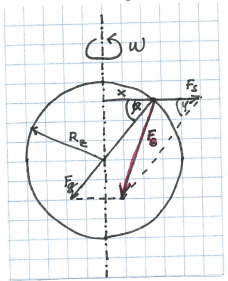
\includegraphics[width=\linewidth]{tihovasila.png}
\end{wrapfigure}%
\begin{align*}
  & \theta ... \text{uhel, ktery siraji vektory} \\[20pt]
  & \vec{F_G}=\vec{F_g}+\vec{F_s} \\
  & F_G^2=F_g^2+F_s+2cos(\theta)F_gF_s \\
  & g^2=G^2\frac{M^2}{R^4}+w^4R^2cos(\theta)^2+2cos(\theta)^2 w^2 G\frac{M^2}{R} \\ 
  & g=<9.78;9.83>\frac{m}{s^2} \\[45pt]
\end{align*}
}
Na povrchu zeme muzeme gravitacni pole aproximovat jako \textbf{homogeni}. V kazdem pripade je vzdy Konzervativni
Diky tomu muzeme definovat tzv \textbf{gravitacni potencial}. Je to energie, potrebna k preneseni telesa o hmotnosti m do bodu A. Pro jedine teleso o hmotnosti m v uzavrene soustave plati
\frm{$\phi=\int_{\infty}^{R}G\frac{m}{r^2} \diff r = -G\frac{m}{R}-(-G\frac{m}{\infty})=-G\frac{m}{R}\\[5pt]
2C=0$}
Pro homogeni gravitacni pole mame $W=E=mgh$ \\
\textbf{Gravitacni silocary} udavaji smer gravitacni sily, \textbf{ekvipotencialni plocha} je plocha, kde s konstantnim gravitacnim potencialem.
\textbf{Pohyby teles v tihovem poli zeme}
\frm{
  $\vec{s}=\frac{1}{2}\vec{a}t^2 +\vec{v}t + \vec{s_0} \\[5pt]
  \vec{a}=\begin{pmatrix}0\\-g \end{pmatrix} \\[5pt]
  \vec{v}=\begin{pmatrix}v_x=v_0 \cos(\theta)\\v_y=v_0\sin(\theta) \end{pmatrix}$
}
doba vystupu do vysky h
\frm{$t_{max}=-(-\frac{2v}{2g})=\frac{v}{g}$}

\cor{\textbf{Keplerovy Zakony}}{
  \begin{enumerate}[label=\bfseries\tiny\protect\circled{\small\arabic*}]
		\item \label{n:1} Planety obíhají kolem Slunce po eliptických trajektoriích, v jejichž jednom společném ohnisku je Slunce. 
    \item \label{n:2} Obsahy ploch opsaných průvodičem planety za stejný čas jsou stejně velké.
    \item \label{n:3} Poměr druhých mocnin oběžných dob dvou planet je stejný jako poměr třetích mocnin délek jejich hlavních poloos. $\frac{T_1^2}{T_2^2}=\frac{a_1^3}{a_2^3}$ ll ll 
\end{enumerate}}
\textbf{Excentricita drahy} je jedna z 6 velicin zvanych elemty drahy, popisujicich presny pohyb planet. Udava typ obezne drahy, druh kuzelosecky. $2a > |F1F2|= 2ea$ e = 0 ... kruznice, 0 < e < 1 ... elipsa e=1 ... parabola, e > 1 ... hyperbola. \\

\begin{figure}[!h]%
    \centering
    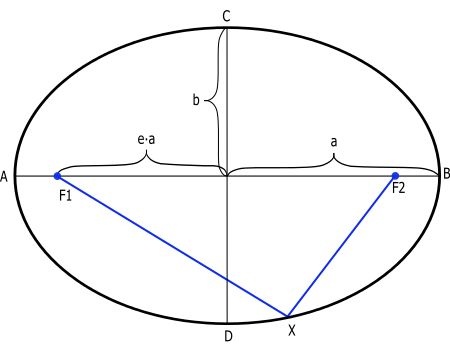
\includegraphics[width=6cm]{images/elipse.png}
    \qquad
    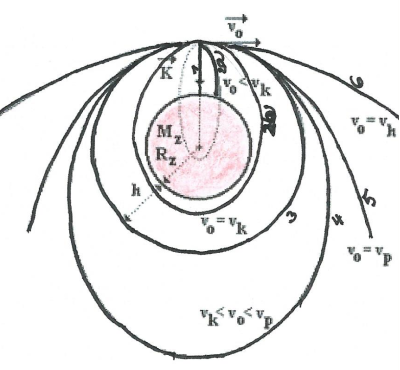
\includegraphics[width=5cm]{images/escape_velocity.png}
\end{figure}
\textbf{Pohyb teles v centralnim gravitacnim poli planety} \\
$v_0$ ... kolmy pad dolu, $v_k$ ... pohyb po kruznici, v < $v_p$ ... pohyb po elipse, $v_p$ ... parabolicka unikova rychlost, $v_h$ ... druha kosmicka rychlost (hyperbola) \\
\newpage

%%%%%%%%%%%%%%%%%%%%%%%%%%%%%%%
% Maturitni otazka 5
%%%%%%%%%%%%%%%%%%%%%%%%%%%%%%

\section{Mechanika tuhého tělesa}
\dfn{Pojmy}{Tuhé těleso, skládání sil v tuhém tělese, moment síly, podmínka rovnováhy tuhého
tělesa, rozklad sil, dvojice sil, těžiště, rovnovážné polohy, otáčivý pohyb tuhého tělesa,
moment setrvačnosti, kinetická energie rotujícího tělesa, [moment hybnosti, pohybová
rovnice pro rotující těleso].}
\vspace{0.5cm}
\textbf{tuhe teleso} = teleso jehoz tvar se nemeni ucinkem libovolne velkych sil. Pohyb takoveho telesa je slozeny ze 2 pohybu: translace, rotace. \\
Newtonovy zakony jednoznacne popisuji, jak se takove teleso pohyhuje, neni to ale prakticky zpusob, jak s nimi zachazet. Proto je potreba zavest nove velicny, ketre lepe vystihnout tento novy otacivy pohyb. \\
\cor{Moment hybnosti}{$L=r \times p$ [$kgm^2/s$]}
\frm{
  $\frac{\diff L}{\diff t} = \dot r \times p + r \times \dot p$ \\[5pt]
$\frac{\diff L}{\diff t} = \frac{p \times p}{m} + r \times f$ \\[5pt]
$\frac{\diff L}{\diff t} = r \times f$ 
}

\cor{Moment sily}{$\frac{\diff L}{\diff t} = M$ [N/m][$kgm^2/s^2$]\hspace{8cm}... ekvivalentni s $\frac{\diff p}{\diff t}=F$}
\textbf{Pro tuhe teleso}
\frm{
\begin{wrapfigure}[11]{L}{5cm}
  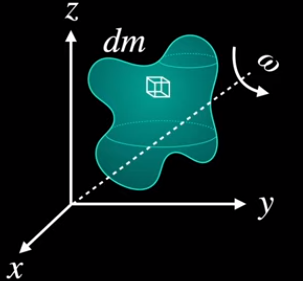
\includegraphics[width=5cm]{images/rigidbody.png}
\end{wrapfigure}%
\begin{align*}
  &dL=r \times dp \text{, } dp = vdm=(w \times r)dm \\
  &L=\int r \times (w \times r) dm \\
  &r \times (w \times r) = 
  \begin{vmatrix}
    \hat x & \hat y  & \hat z \\
    w_x & w_y & w_z \\
    v_x & v_y & v_z
  \end{vmatrix}
  =
  \begin{pmatrix}
   w_x(y^2+z^2)-(w_y xy+w_zxz) \\
   w_y(x^2+z^2)-(w_x xy+w_zyz)\\
   w_z(x^2+y^2)-(w_x xz+w_yyz)
 \end{pmatrix} \\[10pt]
  &L=
  \begin{pmatrix}
    \int (y^2 + z^2) \diff m & - \int xy \diff m & - \int xz \diff m  \\
    - \int xy \diff m & \int  (x^2 + z^2) \diff m & - \int yz \diff m \\
    - \int xz \diff m & - \int yz \diff m & \int (x^2 + y^2) \diff m \\
  \end{pmatrix}
  \begin{pmatrix}
   w_x \\ w_y \\ w_z 
  \end{pmatrix}
\end{align*}
}
\cor{Moment setrvacnosti}{$L_i=I_{ij}w_j$ \hspace{10cm}... ekvivalentni s $p=mv$}

\textbf{Kineticka energie}
\frm{
  $\diff E_k = \frac{1}{2}\diff m v^2=\frac{1}{2} \diff m |w \times r|^2$ \\[10pt]
  $E_k = \int \frac{1}{2}\diff m((w_yz-w_zy)^2+(w_xz-w_zx)^2+(w_xy-w_yx)^2)$ \\[10pt]
  $E_k = \frac{1}{2}\begin{pmatrix} w_x w_y w_z \end{pmatrix}
  \begin{pmatrix}
  I_{xx} & I_{xy} & I_{xz} \\
  I_{yx} & I_{yy} & I_{yz} \\
  I_{zx} & I_{zy} & I_{zz} \\
  \end{pmatrix}
  \begin{pmatrix}
    w_x \\ w_y \\ w_z
  \end{pmatrix}
  = \frac{1}{2}w^TIw=\frac{1}{2}wL$ \\
}
\textbf{Hlavni osy tuheho telesa} : V nasledujicich rovnicich predpokladame, ze osa otaceni prochazi tezistem a zaroven pocatekem.
\frm{
\begin{wrapfigure}[11]{L}{3cm}
  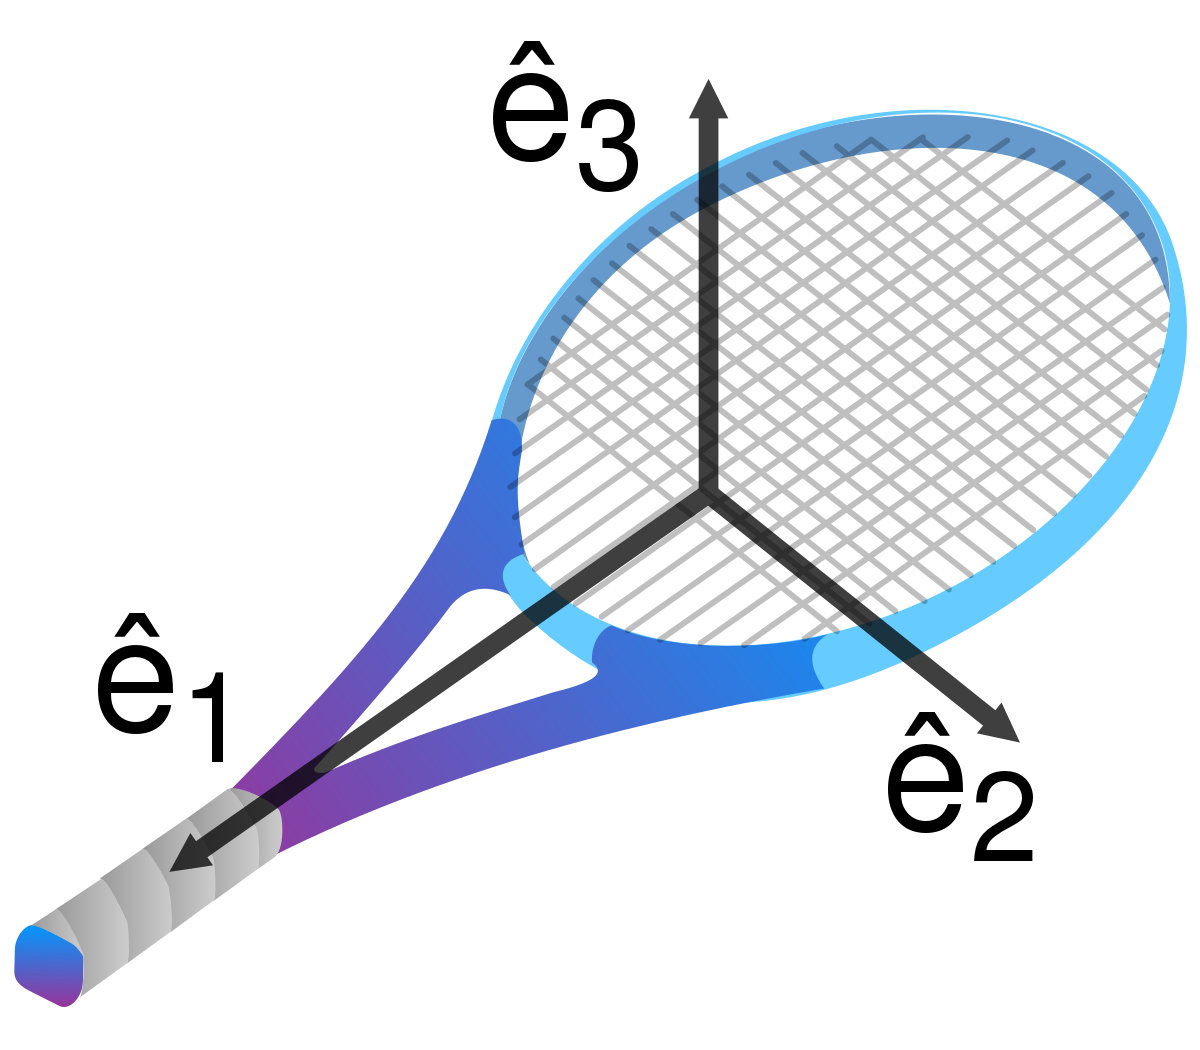
\includegraphics[width=3cm]{images/principal_axis.png}
\end{wrapfigure}%
\begin{align*}
  &[EB]
  \begin{pmatrix}
    I_{xx} & I_{xy} & I_{xz} \\
    I_{yx} & I_{yy} & I_{yz} \\
    I_{zx} & I_{zy} & I_{zz} \\
  \end{pmatrix}_B
  [EB]^T=
  \begin{pmatrix}
    I_{1} & 0 & 0 \\
    0 & I_{2} & 0 \\
    0 & 0 & I_{3} \\
  \end{pmatrix}_E \\[10pt] 
&
\includegraphics[width=5cm]{images/wow.jpeg}
\end{align*}
}
... epicka magie, ktere nerozumim. Kazdemu tuhemu telesu lze najit 3 na sebe kolme osy otaceni(tzn Hlavni osy)(osove vektory baze E), takove, ze pri rotaci je s nimi vektor Momentu Hybnosti rovnobezny, viz eigenvalues, eigenvectors. \\
\textbf{Moment setrvacnosti pro kouli} : ze symetrie koule vyplyva, ze pri totozne uhlove rychlosti, musi byt ve vsech smerech stejne L => $I_1=I_2=I_3=I_{koule}$, $L=I_{koule}w$
\frm{
  \begin{align*}
  I &=\int y^2+z^2 \diff m \\
    &=\rho \int y^2 + z^2 \diff V \\
    &=2 \rho \int_{0}^{R}\int_{0}^{\sqrt{R^2-y^2}} 2\pi r*r^2 \diff r \diff y \\
    &=2 \rho \int_{0}^{R}\frac{1}{2} \pi (R^2 - y^2)^2 \diff y \\
    &= \pi \rho (R^4y-\frac{2}{3}R^2y^3+\frac{1}{5}y^5)\bigg |_{0}^{R} \\
    &= \rho \frac{4}{3} \pi R^3 * \frac{2}{5}R^2 \\
    &=\frac{2}{5} m R^2
  \end{align*}
}

\textbf{rovnovazne polohy} : poloha stala, vratka, volna

\newpage

%%%%%%%%%%%%%%%%%%%%%%%%%%%%%%%
% Maturitni otazka 6
%%%%%%%%%%%%%%%%%%%%%%%%%%%%%%

\section{Mechanika kapalin a plynů}
\dfn{Pojmy}{Struktura tekutin, silové působení mezi částicemi, ideální kapalina a plyn, tlak
v tekutinách, Pascalův zákon, hydrostatický tlak, vztlaková síla, Archimédův zákon,
atmosférický tlak, proudění kapaliny, rovnice kontinuity, Bernoulliova rovnice, vnitřní
tření, proudění reálné kapaliny, obtékání těles, odpor prostředí.}
\vspace{0.5cm}
\textbf{tekutiny = kapaliny + plyny} \\
\textbf{kapaliny} : nestlacitelne, nerozpinave, lisi se mezi sebou vnitrnim trenim \\
\textbf{plyny} : stlacitelne, rozpinave, castice dale od sebe, rychlejsi\\
\textbf{idealni kapalina} dokonale tekuta, bez vnitrniho treni, naprosto neztlacitelna\\
\textbf{idealni plyn} dokonale tekuty, bez vnitrniho treni, dokonale ztlacitelny
\cor{Tlak}{$p=\frac{F}{S}$ [$N/m^2$]}
muze byt vyvolany vnejsi silou : 
\cor{Pascaluv zakon}{Tlak vyvolany vnejsi silou, ktera pusobi na kapalne teleso v uzavrene nadobe, je ve vsech mistech kapaliny stejny}
\textbf{hydraulicka zarizeni} : na zaklade Pascalova zakona meni pomer pusobicich sil 
\frm{$\frac{F_1}{S_1} = \frac{F_2}{S_2}$}
\textbf{hydrostaticky tlak}
\frm{$p = h \rho g$ \hspace{20pt} ... prekvapive plati bez ohledu na tvar nadoby}
ve stejne vysce je v kapaline vsude stejny tlak. Mista o stejnem hydrostatickem tlaku - hladiny \\
\textbf{Atmosfericky tlak} $p\neq h \rho g$, protoze vzduch neni nestlacitelny. Za beznych podminek $p=1013,25 hPa$. Meni se s teplotou vzduchu. Vitr je napriklad zpusobeny rozdilem v tlaku. \\
\textbf{barometr} : nastroj na mereni atmosferickeho tlaku
\textbf{Archimeduv zakon} - tlak na horni plocu telesa je mensi, nez na tu spodni => sila pusobici vzhuru \\
\frm{$F_{vz}=F_{h1}-F_{h2}=V \rho g$ }
... teleso ponorene do kapaliny je nadnaseno silou rovnajici se tize tekutiny stejneho objemu
Na kazde v kapaline tedy pusobi gravitacni a tlakova sila. Jestli se teleso ponori, nebo ne tudiz zalezi na tom jestli je hustota telesa vetsi nez hustota vody.
\textbf{Proudeni kapalin} \\
\textbf{stacionarni} : rychlost kapaliny v danem miste zustava konstanti s casem \\
\textbf{nestacionarni} : rychlost se meni \\
\textbf{laminarni} : proudnice rovnobezne \\
\textbf{turbulentni} : chaoticke \\
\cor{Objemovy prutok}{$Q_v=\frac{V}{t}=\frac{Sl}{t}=Sv$ [$m^3/s$]}
Kvuli nestlacitelnosti kapaliny musi byt objemovy prutok trubice ve vsech mistech stejny, bez ohledu na rozsirovani, nebo zuzeni. \\
\cor{Bernouliho rovnice}{
hydrostaticky tlak je ve stejnych hloubkach stejny jen za predpokladu ze je kapalina v klidu. \\
pro proudici kapalinu plati jine zakonitosti. Lze popsat pomoci Zakonu zachovani energie. My se, ale budeme zabyvat jen stacionarnim proudenim kapalin \\[10pt]
$E=E_k+E_p$ \\[10pt]
pri zmene rychlosti proudici kapaliny ve zuzeni/rozsireni trubice se musi zachovat jeji celkova energie. Je tudiz potreba definovat novou tlakovou potencialni energii. \\[10pt]
$E_p=\int p\vec{S}d\vec{l}=pV+\int \dot{p} V dl = pV$  \\[10pt]
... proudeni je stacionarni, tkaze p se nemeni s casem. My ho navic povazujeme za konstantni v jednotlivych usecich nadoby(trubky) \\[10pt]
$E_k=\frac{1}{2}mv^2=\frac{1}{2} \rho V v^2$
}
\frm{
  \begin{wrapfigure}[11]{L}{5cm}
    \vspace*{-0.2cm}
    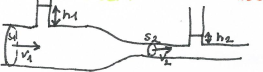
\includegraphics[width=\linewidth]{images/bernouli.png}
  \end{wrapfigure}%
  \begin{align*}
    p_1+\frac{1}{2}\rho v_1^2=p_2+\frac{1}{2}\rho v_2^2 \\ 
  \end{align*} 
}
\newpage

%%%%%%%%%%%%%%%%%%%%%%%%%%%%%%%
% Maturitni otazka 7
%%%%%%%%%%%%%%%%%%%%%%%%%%%%%%

\section{Základní pojmy molekulové fyziky a termodynamiky}
\dfn{Pojmy}{Kinetická teorie látek, Brownův pohyb, difúze, interakce mezi částicemi, modely struktur
skupenství, látkové množství, Avogadrova konstanta, molární veličiny, stavové veličiny,
rovnovážný stav, nultý termodynamický zákon, rovnovážný děj, vratný děj, vnitřní
energie.}
\vspace{0.5cm}
\cor{Kinetikcka teorie latek}{teorie, ktera objasnuje strukturu a vlastnosti latek pohybem a vzajemnym pusobenim atomu molekul a iontu, z nichz  se latky skladaji.

  \begin{enumerate}[label=\bfseries\tiny\protect\circled{\small\arabic*}]
  \item \label{n:1} Vsechny latky(kterehokoliv skupenstvi) jsou slozeny z castic (atomy, molekuly, ionty). Mezi casticemi jsou mezery, proto mluvime o nespojite (diskretni strukture latek)
    \item \label{n:2} Tyto castice se neustale a neusporadane pohybuji (=tepelny pohyb) => maji kinetickou energii
  \end{enumerate}
}
o tepelnem pohybu castic v latkach svedci mnohe jevy \\
\textbf{Difuze} : samovolny pohyb molekul rozpustene latky z mista o vyssi koncentraci do mista s nizsi koncentraci. Za urcitou dobu se daa latka rpz[ty li do celeho objemu rooztoku a jeji koncetrace bude vsude stejna \\
\textbf{Brownuv pohyb} : nepretrzity a chaoticky pohyb mikroskopickych castic v plynne, nebo kapalnem mediu. Rychlost Brownova pohybu je umerna teplote systemu.  \\
\cor{...}{
  \begin{enumerate}[label=\bfseries\tiny\protect\circled{\small\arabic*}]
    \setItemnumber{3}
    \item \label{n:3}{Castice na sebe pusobi silami elektromagneticke povahy - pritazlive, odpudive}
  \end{enumerate}
}

\begin{wrapfigure}[7]{r}{0.4\textwidth}
  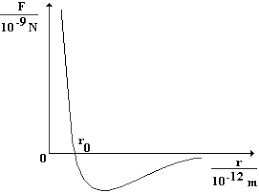
\includegraphics[width=0.4\textwidth]{kinetic_theory.png}
\end{wrapfigure} 
vzajemne silove pusobeni mezi dvema casticemi v zavislosti na vzdalenosti mezi nimi  \\[10pt]
  $\bullet$ \textbf{sfera vzajemneho pusobeni} : kazda castice je pritahovana jen nejblizsimi casticemi ve svem okoli \\
  $\bullet$ \textbf{vazebne sily}  sily jimiz na sebe pusobi atomy v molekule \\
  $\bullet$ kvuli silovym pusobenim mezi casticemi ma teleso i vnitrnipotencialni energii\\
  $\bullet$ $r_0$ : rownovazna poloha, nepusobi sila \\
  \vspace{2cm}
  
  \textbf{Stavove veliciny} : veliciny, ktere popisuji stav termodynamickeho systemu. Deli se na: \\
  \textbf{extenzivni} : zavisi na velikosti systemu \\
    Objem ,
    Hmotnost , 
    Latkove mnozstvi ,
    Vnitrni energie, entalpie, dalsi termodynamicke potencialy , 
    Entropie \\
  
  \textbf{intenzivni}: jsou na velikosti systemu nezavisle \\
    Tlak ,
    Teplota ,
    Hustota \\ 

  \cor{Molarni Veliciny}{
    \textbf{atomova hmotnostni jednotka} : $\frac{1}{12}$ hmotnosti atomu uhliku nuklidu $C^{12}$ $m_u = 1.66*10^{-27} $ [kg] \\
    \textbf{Relativni aromova hmotnost $A_r$} - udava kolikrat je atom tezsi,
    $m=A_rm_u$ \\[10pt]
    \textbf{Avogadrova konstanta} - pocet castic v jednom molu
    $N_A=6.02*10^{23} $ $[mol^{-1}]$ \\
    \textbf{Latkove Mnozstvi $n$} - vyjadruje pocet castic v telese v molech 
    $N=N_A*n$ \\[10pt]
    \textbf{Molarni hmotnost $M_m$} : hmotnost 1 molu latky 
    $m=M_mn$ [$kg/mol$] \\
    \textbf{Molarni objem $V_m$} : objem 1 molu latky 
    $V=V_mn$ [$m^3/mol$]\\ 
    \textbf{molarni objem plynu} za normalnich podminek, tzn $V_m=22,414$ [$l$]
    $1,66*10^{-27}*6.02*10^{23}=10^{-3}$ \hspace{2cm} ... nahoda? ne, picus chemik prohlasil gram za hlavni jednotku \\
  }
  \textbf{Chemicka vazba} : spojeni mezi atomy s nestabilni elektronovou konfiguraci => tvori molekuly
  \textbf{krystalova mrizka} : mnozina urcitych abstraktnich bodu, podle nichz se popisuje struktura krystalu
  \cor{Vnitrni energie}{soucet vsech kinetickych a potencialnich energie\\}
\cor{Teplo}{energie, kterou pri tepelne vymene preda teleso s vyssi teplotou \\[5pt]
  $Q=mc \Delta t$ [$J$]\\[5pt]
  \textbf{merna tepelna kapcita $c$} [$J/kgK$]
}
\textbf{Rovnovazny stav soustavy} : každá soustava, která je od určitého okamžiku v neměnných vnějších podmínkách, přejde samovolně po určité době do rovnovážného stavu a samovolně z něho nevyjde.\\
\textbf{Rovnovážný děj} je děj, při kterém soustava prochází řadou na sebe navazujících rovnovážných stavů. Reálné děje lze považovat za rovnovážné, probíhají-li dostatečně pomalu.
\ex{}{
Když píst s plynem rychle stlačíme, potřebuje plyn na dosažení rovnováhy určitý čas
(molekuly na druhé straně neví, že píst je stlačován, dokud k nim nedorazí vytlačené
molekuly => chvíli trvá než se vytlačené molekuly rozmístí po pístu a vyrovná se tlak a
teplota v celém objemu).
Stlačujeme pomaleji: vytlačených molekul je méně, rozdíly v tlaku jsou menší => pokud
budeme píst stlačovat dostatečně pomalu, bude mít teplota i tlak dost času na vyrovnání
v celém objemu => v každém okamžiku se plyn bude chovat, jako kdyby byl v rovnovážné
poloze => rovnovážný děj. 
}
\textbf{Modely jednotlivych skupenstvi} 
\begin{enumerate}[label=\bfseries\tiny\protect\circled{\small\arabic*}]
  \item \textbf{pevne latky} castice blizko u seb, pravidelne usporadany 
  \item \textbf{kapaliny} castice dal od sebe  
  \item \textbf{plyny} castice nejdal od sebe  
\end{enumerate}
\newpage

%%%%%%%%%%%%%%%%%%%%%%%%%%%%%%%
% Maturitni otazka 8
%%%%%%%%%%%%%%%%%%%%%%%%%%%%%%

\section{Vnitřní energie, teplo, teplota}
\dfn{Pojmy}{Vnitřní energie, změny vnitřní energie (práce, tepelná výměna), první termodynamický
zákon, tepelná rovnováha, teplota, teplotní stupnice, třetí termodynamický zákon, měrná
tepelná kapacita, kalorimetrická rovnice, přenos vnitřní energie (vedením, prouděním,
zářením).}
\newpage

%%%%%%%%%%%%%%%%%%%%%%%%%%%%%%%
% Maturitni otazka 9
%%%%%%%%%%%%%%%%%%%%%%%%%%%%%%

\section{Struktura a vlastnosti plynů}
\dfn{Pojmy}{Model ideálního plynu, rozdělení molekul podle rychlosti, střední kvadratická rychlost,
střední kinetická energie molekuly, teplota a tlak plynu, stavová rovnice pro ideální plyn,
Avogadrův zákon, normální molární objem, tepelné děje s ideálním plynem a jejich
grafické vyjádření, kruhový děj, Carnotův cyklus, tepelné a chladící stroje, druhý
termodynamický zákon.}
\newpage

%%%%%%%%%%%%%%%%%%%%%%%%%%%%%%%
% Maturitni otazka 10
%%%%%%%%%%%%%%%%%%%%%%%%%%%%%%

\section{Struktura a vlastnosti pevných látek}
\dfn{Pojmy}{Stavba látek z částic, silové působení mezi částicemi, druhy vazeb, látky amorfní a
krystalické, model krystalové mřížky, poruchy v krystalové mřížce, deformace,
normálové napětí, relativní prodloužení, Hookův zákon, křivka deformace, teplotní
roztažnost.}
\newpage

%%%%%%%%%%%%%%%%%%%%%%%%%%%%%%%
% Maturitni otazka 11
%%%%%%%%%%%%%%%%%%%%%%%%%%%%%%

\section{Struktura a vlastnosti kapalin}
\dfn{Pojmy}{Povrchová vrstva kapalin, povrchová energie, povrchové napětí, povrchová síla, jevy na
rozhraní, kapilární tlak, kapilární jevy, teplotní roztažnost kapalin.}
\newpage

%%%%%%%%%%%%%%%%%%%%%%%%%%%%%%%
% Maturitni otazka 12
%%%%%%%%%%%%%%%%%%%%%%%%%%%%%%

\section{Skupenské přeměny látek}
\dfn{Pojmy}{Fázový diagram, trojný a kritický bod, modely struktury skupenství, vnitřní energie a její
změny při změnách skupenství, vypařování, kondenzace, sytá pára, přehřátá pára, var,
sublimace, tání, tuhnutí, měrné skupenské teplo přeměny, vlhkost vzduchu.}
\newpage

%%%%%%%%%%%%%%%%%%%%%%%%%%%%%%%
% Maturitni otazka 13
%%%%%%%%%%%%%%%%%%%%%%%%%%%%%%

\section{Mechanické kmity}
\dfn{Pojmy}{Pohyb kmitavý, periodický, harmonický, kinematika harmonického pohybu (výchylka,
rychlost, zrychlení, fáze, frekvence, perioda), skládání kmitů v jedné přímce, skládání
kmitů navzájem kolmých, Lissajousovy obrazce, dynamika harmonického pohybu,
pružina, kyvadlo, přeměny energie v oscilátorech, tlumené kmity, nucené kmity,
rezonance.}
\newpage

%%%%%%%%%%%%%%%%%%%%%%%%%%%%%%%
% Maturitni otazka 14
%%%%%%%%%%%%%%%%%%%%%%%%%%%%%%

\section{Mechanické vlnění}
\dfn{Pojmy}{Vznik, šíření a druhy vlnění (postupné, stojaté, příčné, podélné), rychlost šíření vlny
(fázová rychlost), vlnová délka, rovnice postupné vlny, interference vlnění, koherentní
vlnění, odraz vlnění, Huygensův princip, zákon odrazu s lomu, ohyb vlnění, zvuk,
Dopplerův jev, souvislosti s optikou.}
\newpage

%%%%%%%%%%%%%%%%%%%%%%%%%%%%%%%
% Maturitni otazka 15
%%%%%%%%%%%%%%%%%%%%%%%%%%%%%%

\section{Elektrostatické pole}
\dfn{Pojmy}{Elektrický náboj, zákon zachování náboje, Coulombův zákon, elektrostatické pole,
homogenní a radiální pole, intenzita elektrického pole, elektrický potenciál, elektrické
napětí, práce v homogenním elektrickém poli, vodič a nevodič v elektrickém poli,
elektrostatická indukce, kapacita vodiče, kapacita soustavy vodičů, kondenzátory, řazení
kondenzátorů.}
\newpage

%%%%%%%%%%%%%%%%%%%%%%%%%%%%%%%
% Maturitni otazka 16
%%%%%%%%%%%%%%%%%%%%%%%%%%%%%%

\section{Elektrický proud v kovech}
\dfn{Pojmy}{Elektrický proud, elektromotorické napětí, elektronová vodivost, Ohmův zákon,
voltampérová charakteristika, elektrický odpor, závislost odporu na rozměrech vodiče a
na teplotě, supravodivost, termočlánek, Ohmův zákon pro uzavřený obvod, vnitřní odpor
zdroje, Kirchhoffovy zákony, výkon elektrického proudu.}
\newpage

%%%%%%%%%%%%%%%%%%%%%%%%%%%%%%%
% Maturitni otazka 17
%%%%%%%%%%%%%%%%%%%%%%%%%%%%%%

\section{Elektrický proud v polovodičích}
\dfn{Pojmy}{Polovodiče vlastní, příměsové, typ N, typ P, přechod PN, diodový jev, dioda jako
usměrňovač, Graetzovo zapojení, tranzistorový jev, tranzistor jako zesilovač, termistory,
diody LED, fotodiody.}
\newpage

%%%%%%%%%%%%%%%%%%%%%%%%%%%%%%%
% Maturitni otazka 18
%%%%%%%%%%%%%%%%%%%%%%%%%%%%%%

\section{Elektrický proud v kapalinách a plynech}
\dfn{Pojmy}{Elektrolytická disociace, elektrolýza, závislost proudu v elektrolytu na napětí, Faradayovy
zákony elektrolýzy, galvanické články, elektrolytická polarizace, akumulátory, ionizace,
nesamostatný a samostatný výboj, voltampérová charakteristika výboje, doutnavý výboj,
jiskra, oblouk, katodové záření, elektronový paprsek, emise elektronů.}
\newpage

%%%%%%%%%%%%%%%%%%%%%%%%%%%%%%%
% Maturitni otazka 19
%%%%%%%%%%%%%%%%%%%%%%%%%%%%%%

\section{Stacionární magnetické pole}
\dfn{Pojmy}{Magnetické pole elektrického proudu, magnetické indukční čáry, Ampérovo pravidlo,
magnetická indukce, magnetické pole vodičů s proudem, silové působení na náboje a
vodič s proudem, Flemingovo pravidlo, silové působení mezi dvěma vodiči s proudem,
definice ampéru, magnetické vlastnosti látek (diamagnetické, paramagnetické,
feromagnetické), magnetická hystereze (látky magneticky měkké a tvrdé).}
\newpage

%%%%%%%%%%%%%%%%%%%%%%%%%%%%%%%
% Maturitni otazka 20
%%%%%%%%%%%%%%%%%%%%%%%%%%%%%%

\section{Nestacionární magnetické pole}
\dfn{Pojmy}{Elektromagnetická indukce, Faradayův zákon elektromagnetické indukce, magnetický
indukční tok, Lenzův zákon, Foucaultovy proudy, vlastní indukce, indukčnost,
přechodové děje.}
\newpage

%%%%%%%%%%%%%%%%%%%%%%%%%%%%%%%
% Maturitni otazka 21
%%%%%%%%%%%%%%%%%%%%%%%%%%%%%%

\section{Střídavé elektrické proudy}
\dfn{Pojmy}{Vznik střídavého proudu, generátory, napětí fázové a sdružené, elektromotory,
transformátor, harmonický průběh střídavého proudu, obvody s R, L, C, sériový a
paralelní kmitavý obvod (rezonance), výkon střídavého proudu, [řešení obvodů pomocí
komplexních čísel].}
\newpage

%%%%%%%%%%%%%%%%%%%%%%%%%%%%%%%
% Maturitni otazka 22
%%%%%%%%%%%%%%%%%%%%%%%%%%%%%%

\section{Elektromagnetické pole, kmity, vlnění}
\dfn{Pojmy}{Kmitavý obvod jako zdroj elektromagnetického pole, vznik elektromagnetického vlnění,
elektromagnetický dipól, vysílač, přijímač, sdělovací technika (mikrofon, reproduktor,
modulace, rozhlas, televize), spektrum elektromagnetického vlnění.}
\newpage

%%%%%%%%%%%%%%%%%%%%%%%%%%%%%%%
% Maturitni otazka 23
%%%%%%%%%%%%%%%%%%%%%%%%%%%%%%

\section{Geometrická optika}
\dfn{Pojmy}{Šíření světla, optické prostředí, [Fermatův princip], zákon odrazu a lomu světla, rozklad
(disperze) světla, optická soustava, zrcadla, čočky, zobrazovací rovnice, příčné zvětšení,
oko, optické přístroje.}
\newpage

%%%%%%%%%%%%%%%%%%%%%%%%%%%%%%%
% Maturitni otazka 24
%%%%%%%%%%%%%%%%%%%%%%%%%%%%%%

\section{Vlnová optika}
\dfn{Pojmy}{Spektrum elektromagnetického vlnění, vznik a podstata světla, šíření světla, Huygensův
princip, odraz, lom, interference světla, koherence, Youngův pokus, interference na tenké
vrstvě (Newtonova skla), holografie, ohyb světla, polarizace.}
\newpage

%%%%%%%%%%%%%%%%%%%%%%%%%%%%%%%
% Maturitni otazka 25
%%%%%%%%%%%%%%%%%%%%%%%%%%%%%%

\section{Fotometrie}
\dfn{Pojmy}{Zářivý tok (světelný tok), zářivost (svítivost), ozáření (osvětlení), tepelné záření, záření
černého tělesa, Stefan-Boltzmanův zákon, Wienův posunovací zákon, Planckův zákon,
kvantum energie, spektrum elektromagnetického záření (UV, RTG, $\gamma$)}
\newpage

%%%%%%%%%%%%%%%%%%%%%%%%%%%%%%%
% Maturitni otazka 26
%%%%%%%%%%%%%%%%%%%%%%%%%%%%%%

\section{Základy speciální teorie relativity}
\dfn{Pojmy}{Inerciální soustavy, Galileiho princip relativity, Michelson - Morley, Einsteinovy
postuláty, Lorentzova transformace, relativnost současnosti, dilatace času, kontrakce
délek, skládání rovnoběžných rychlostí, relativistická hmotnost, relativistická hybnost,
relativistická energie (E=mc2).}
\newpage

%%%%%%%%%%%%%%%%%%%%%%%%%%%%%%%
% Maturitni otazka 27
%%%%%%%%%%%%%%%%%%%%%%%%%%%%%%

\section{Základy kvantové fyziky}
\dfn{Pojmy}{Kvantování energie (Planck), fotoelektrický jev (Einsteinova rovnice, foton), Comptonův
jev, vlnové vlastnosti částic (de Broglieovy vlny), korposkulárně vlnový dualismus,
Davisson-Germerův pokus, [Schrödingerova rovnice], Heisenbergovy relace neurčitosti,
kvantování fyzikálních veličin, princip korespondence.}
\newpage

%%%%%%%%%%%%%%%%%%%%%%%%%%%%%%%
% Maturitni otazka 28
%%%%%%%%%%%%%%%%%%%%%%%%%%%%%%

\section{Fyzika elektronového obalu}
\dfn{Pojmy}{Modely atomu, spektrum vodíku, Franck-Hertzovy pokusy, kvantově mechanický model
atomu vodíku, kvantová čísla, orbitaly, spin, Pauliho princip, elektronová konfigurace,
periodická soustava prvků, emise světla, laser.}
\newpage

%%%%%%%%%%%%%%%%%%%%%%%%%%%%%%%
% Maturitni otazka 29
%%%%%%%%%%%%%%%%%%%%%%%%%%%%%%

\section{Fyzika atomového jádra}
\dfn{Pojmy}{Modely atomového jádra, jaderné síly, závislost vazebné energie připadající na jeden
nukleon na nukleonovém čísle, hmotnostní úbytek, radioaktivita, zákon radioaktivní
přeměny (rozpadu), poločas rozpadu, rozpadové řady, umělá radioaktivita, jaderné reakce,
jaderná energetika, detektory částic, urychlovače částic.}


\end{document}
